\chapter{Introduction}
In the early days of AI, researchers utilised traditional programming techniques to simulate intelligent behaviour in machines. This meant that the ability of machines to perform complex tasks depended on the ability of humans to express solutions to those tasks in the form of precisely defined computational steps. This fundamental limitation led to the development of mathematical methods that allow programs to learn from experience, as opposed to following explicit instructions. These approaches are encapsulated in the field of Machine Learning (ML), which has risen to the forefront of AI research.

Recently, Neural Networks - a class of ML algorithms that loosely resemble the structure of biological neural networks in the brain - have gained a lot of popularity. Due to the growing availability of data and computational power, these algorithms have achieved comparable (and often superior) performance to humans at complicated tasks, from recognising faces to driving automobiles. One area in particular in which neural networks have shown extraordinary results is Reinforcement Learning (RL). RL is a technique in which a ML algorithm, called an agent, learns to operate in an environment (e.g. a video game) by interacting with it. The agent is allowed to operate freely in the environment, while trying to maximise some notion of a reward that its creators have defined.

Despite their usefulness, neural networks have important limitations. One such limitation is the issue of uninterpretability: the solutions produced by neural networks are too complicated for humans to understand. This problem is of particular importance in RL because our inability to understand an agent’s decision-making process makes it difficult to replicate desirable behaviours and prevent undesirable ones. Additionally, this problem presents an issue in morally significant situations. For example, imagine a medical AI tasked with diagnosing severe conditions in patients. Given its inability to explain its thought process, it would be difficult for patients to be convinced to make big life decisions based on the information they are given.

Many recent attempts have been made that used traditional AI techniques, such as Genetic Programming (GP), to tackle the problem of interpretability. GP is a technique that borrows concepts from biological evolution to automatically generate programs that solve a given problem. In most of these attempts, GP was used in combination with neural networks to produce solutions that perform well while, at the same time, offering a degree of interpretability. The limitation of these approaches is that uninterpretability cannot be eliminated as long as neural networks are part of the process. That’s why, in this project, GP was used directly as a standalone alternative to neural-network-based techniques, to produce solutions in the form of human-readable programs that achieve competitive performance in various RL tasks. 

The project began by applying GP to a simple classic control environment called cart-pole, in which the goal is to balance a wooden pole on a flat rectangular surface (figure \ref{fig:cart-pole}). I manually discovered a strategy for beating the game by interacting with the environment, and then I implemented a GP algorithm to automatically find a program that implements this strategy. After this experiment was successful, I wanted to apply the same algorithm to an environment that was similar enough to cart-pole but less constrained, and therefore more difficult to solve, to establish a baseline of problems of increasing difficulty that this algorithm would be able to tackle. So, I picked another popular ML benchmark called mountain-car, which simulates a vehicle attempting to climb a steep hill (figure \ref{fig:mountain-car}). I did not guide the algorithm to a known strategy this time, but instead implemented the required extensions to allow it to discover one by itself. The results were again positive: it was much easier for the algorithm to converge on a well-performing, and still interpretable, solution than I was expecting. Finally, I applied the algorithm on the inverted pendulum environment (figure \ref{fig:pendulum}), which needs to be swung until it points upwards and then balanced there for as long as possible. This environment is structurally similar to mountain-car, with the added difficulty of requiring to maintain the achieved state (pointing upwards) as opposed to simply reaching it. The GP algorithm managed to discover strategies that performed reasonably well and which, after being interpreted, were manually improved to eventually achieve performance close to the best neural-network-based solutions, without a loss in interpretability.

\begin{figure}[H]
    \centering
    \includegraphics[width=3.8cm]{images/cartpole}
    \caption{Cart-Pole}
    \label{fig:cart-pole}
\end{figure}

\begin{figure}[H]
    \centering
    \includegraphics[width=3.8cm]{images/mountain-car}
    \caption{Mountain-Car}
    \label{fig:mountain-car}
\end{figure}

\begin{figure}[H]
    \centering
    \includegraphics[width=3.8cm]{images/pendulum}
    \caption{Pendulum}
    \label{fig:pendulum}
\end{figure}

% \includegraphics[width=3.8cm]{cartpole.png}
% \includegraphics[width=3.8cm]{mountain-car.png}
% \includegraphics[width=3.8cm]{pendulum.png}

\section{Report Overview}
This report is structured in chapters. Chapter 1 includes the introduction and this overview section. Chapter 2 covers the professional considerations that need to be taken into account according to the BCS code of conduct. Chapter 3 provides background information on the technical topics relevant to the project, namely Machine Learning and Genetic Programming, as well as an overview of related work, and explains how the approach used in this project differs from other approaches. Chapter 4 discusses the methods used in the project, including details about the experiments performed and pseudocode to encourage replication. Chapters 5 and 6 cover the experiments performed using the RL environments (cart-pole, mountain-car, and pendulum, in that order) and the results obtained for each of them. Chapter 7 provides a conclusion as well as a discussion of the limitations of this project and suggestions for future extensions.
